\documentclass[a4paper,10pt]{article}
\usepackage[utf8]{inputenc}
\usepackage{float}
\usepackage{graphicx}

%opening
\title{Particle pusher interface}
\author{Otto Hannuksela}

\begin{document}

\maketitle

\tableofcontents

\newpage

\section{Setup}

\subsection{Edit paths}

\begin{verbatim}
 cd ~/analysator
 gedit pyMayavi/particlepusherinterface.py
\end{verbatim}

Locate the following and change the paths (/home/otto to e.g. /home/sanni) to vlasiator path:

\begin{verbatim}
   #Executable location
   parse_args.append("/home/otto/vlasiator/particle_post_pusher")
   # Options
   parse_args.append("--run_config")
   # CFG location
   parse_args.append("/home/otto/vlasiator/particles/particles.cfg")
\end{verbatim}

Note: you must have particle\_post\_pusher compiled:

\begin{verbatim}
 cd ~/vlasiator
 make particle_post_pusher
\end{verbatim}


\subsection{Edit particle pusher cfg}

\begin{verbatim}
 # Change to Vlasiator path:
 cd ~/vlasiator/particles
 gedit particles.cfg
\end{verbatim}

Now we want to set up the paths to vlsv files we are using in our analysis

Locate and edit the following in particles.cfg to local paths:

\begin{verbatim}
input_filename_pattern = /lustre/tmp/alfthan/2D/sisu_equatorial_7/bulk.%07i.vlsv
\end{verbatim}

Make sure mode = analysator (as follows):
\begin{verbatim}
mode = analysator
\end{verbatim}

Set up the starting and ending time (particles will be propagated from starting time to ending time:

\begin{verbatim}
# Starting time of the particles (in seconds)
start_time = 1488
end_time = 2976
\end{verbatim}

Thats it!

\section{Using the particle pusher interface}

Ipython example:

Starting up the particle pusher (Use VlasiatorReader, not VlsvReader):

\begin{verbatim}
ipython

In [2]: import pytools as pt

In [3]: f = pt.vlsvfile.VlasiatorReader('bulk.0001480.vlsv')

In [4]: grid = pt.grid.Particlepusherinterface(f, 'rho')
\end{verbatim}

\subsection{Using the particle pusher options}

The usage is illustrated in the Figures \ref{fig:particle1} and \ref{fig:particle2}.

\begin{figure}[H]
 \centering
 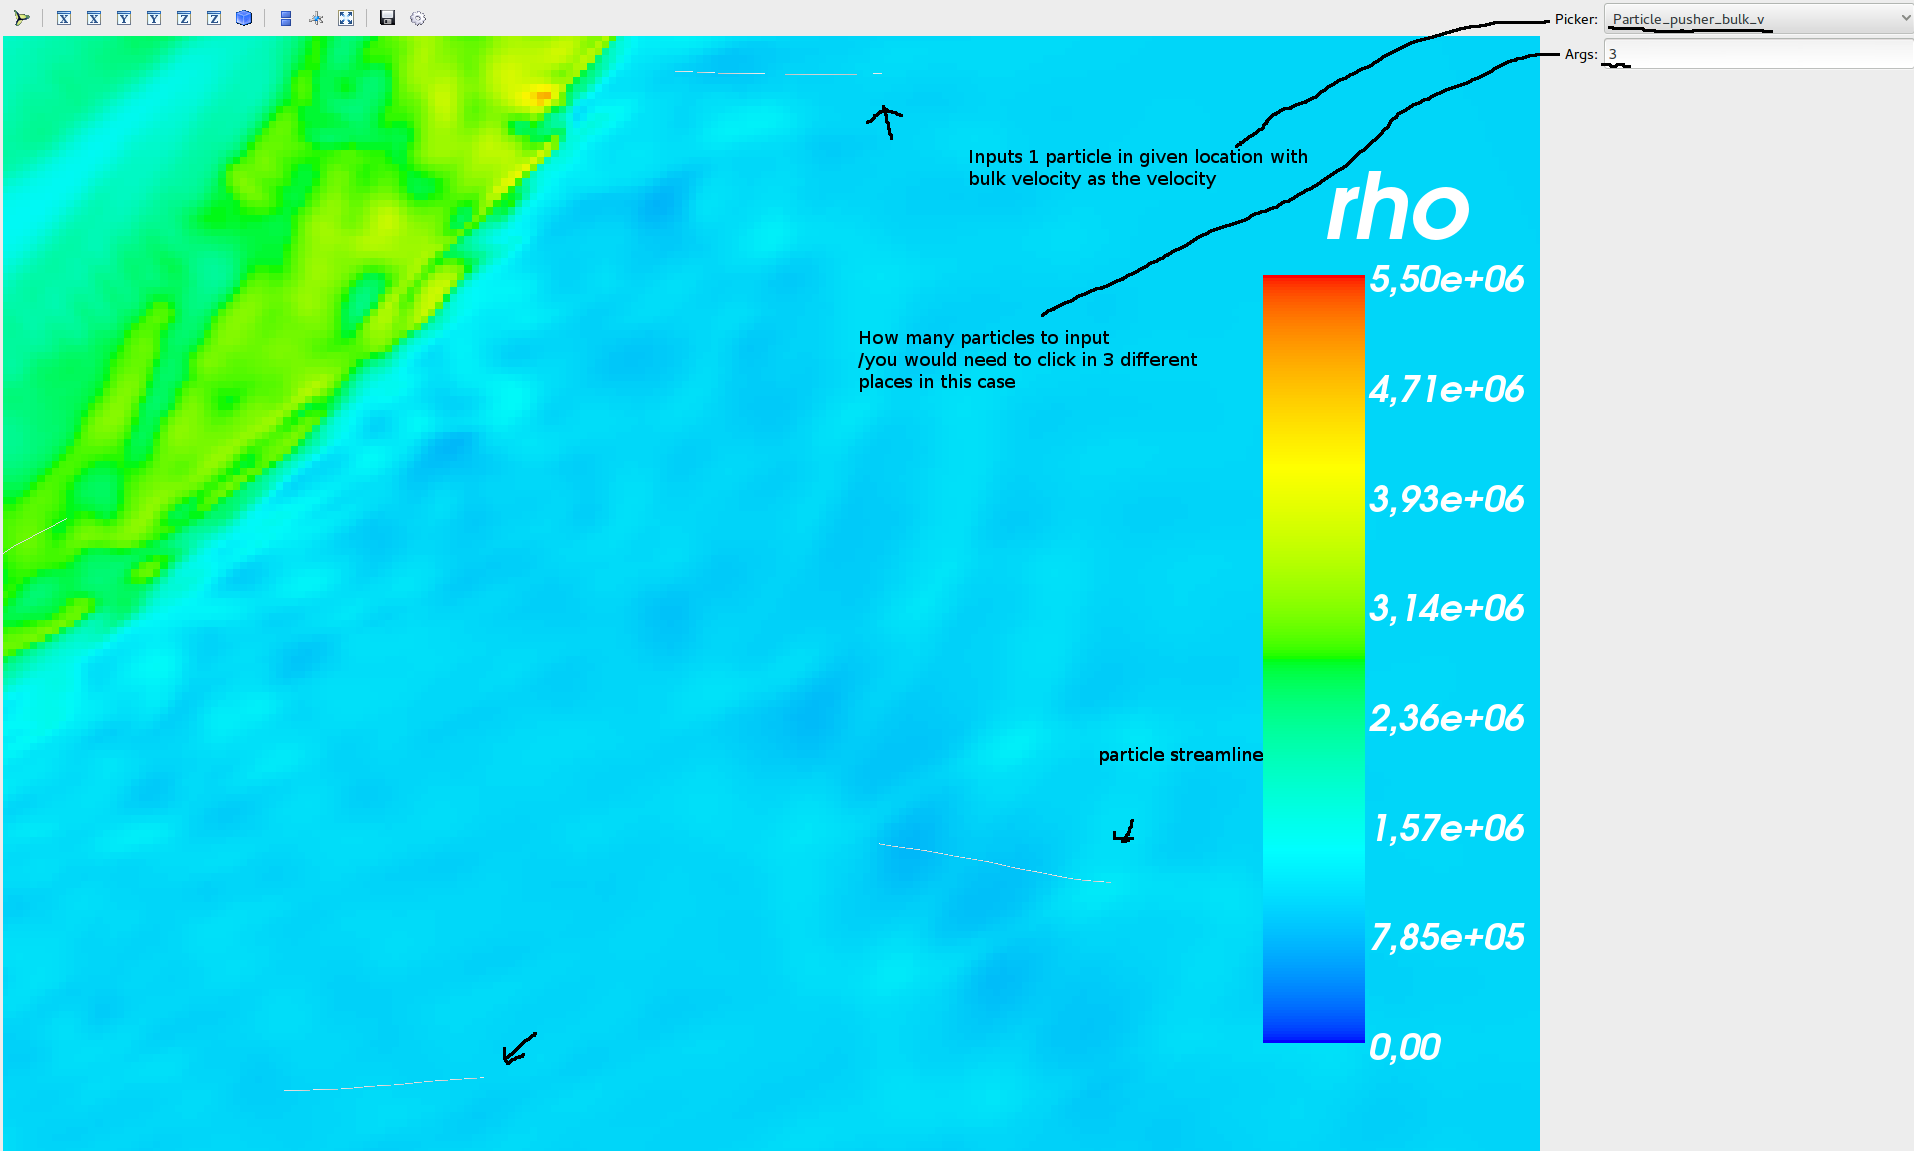
\includegraphics[width=\textwidth]{./images/particlepusherbulk.png}
 \caption{Particle pusher usage for bulk velocity sampling}
 \label{fig:particle1}
\end{figure}

\begin{figure}[H]
 \centering
 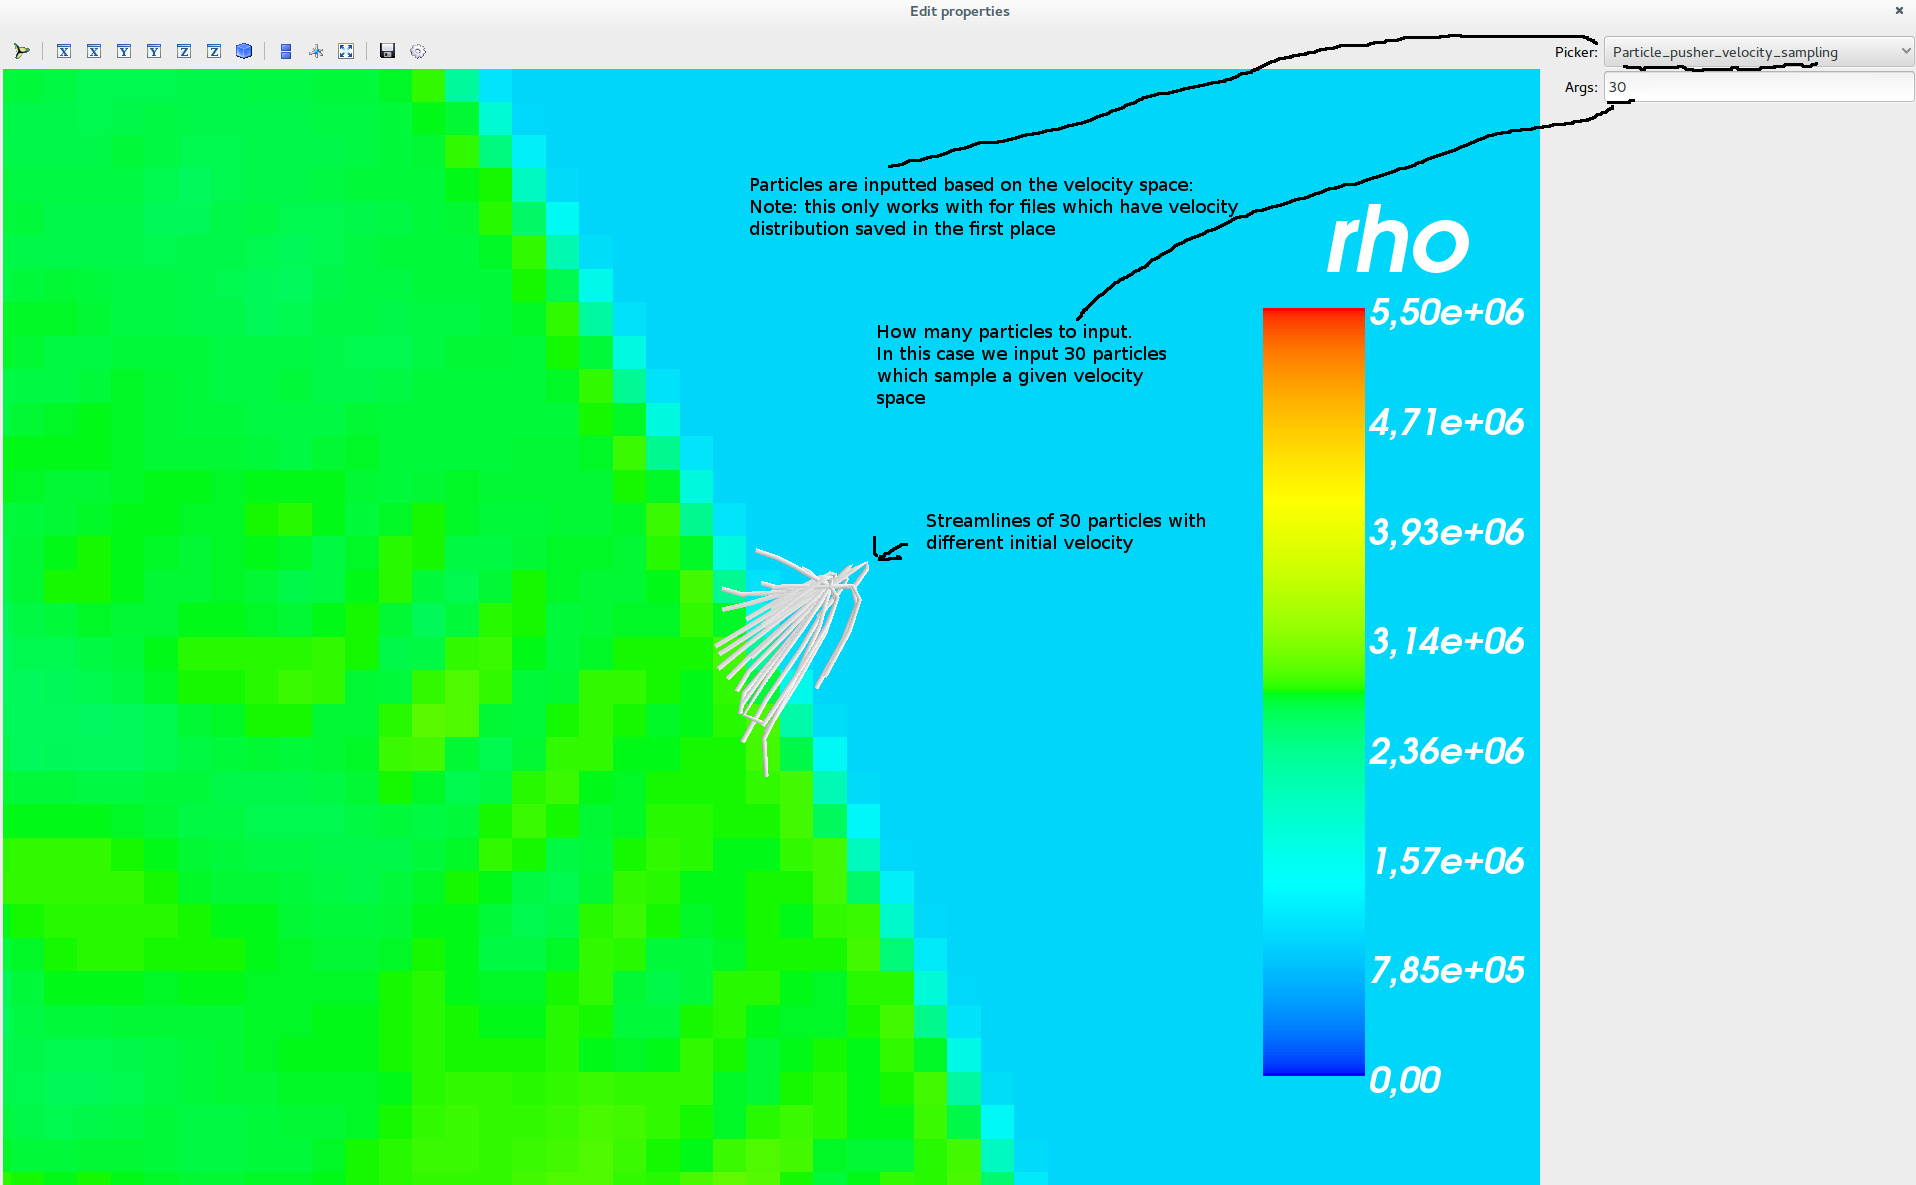
\includegraphics[width=\textwidth]{./images/particlepushersampling.png}
 \caption{Particle pusher usage for velocity space sampling}
 \label{fig:particle2}
\end{figure}


\end{document}
